\documentclass[letterpaper,11pt]{article}
%--------------Document configuration begins--------------
\usepackage{fullpage}
\usepackage[numbers]{natbib} 	%\citet{jon90} --> Jones et al. [21], \citep{jon90} --> [21]
\usepackage[colorlinks]{hyperref}
%--------------Document configuration ends--------------

%Import personal commands 
\usepackage{commandscsp}		

%Load cleveref last
\usepackage{amsthm}
\usepackage[capitalize]{cleveref}
\usepackage{commands_theo} 			%Theorems, lemmas, proofs, etc

\title{\vspace{-1cm} \bf Constrained Shortest Path \vspace{-1.3cm}}
\author{}
\begin{document}
\maketitle


\section{Average HD}\label{sec:avg_hd}

We relax the definition of HD in two ways.
First, a LSHS needs to be locally sparse just ``in average''.
Second, we forget the strong limitation of hitting $S_r(v,\calQ)$ and ask only for the existence of a multiscale LSHS.

\begin{definition}[Average LSHS]
Given $r>0$ and a system $\calQ$, a set $C\subseteq V$ is an average $(h,r)$-LSHS if it hits $\calQ_r$ and is locally sparse in average, i.e.,
\[
\frac{1}{n}\sum_{v\in V} \abs{B_{2r}(v)\cap C} \leq h.
\]
\end{definition}

\begin{definition}[Average HD]
The system $\calQ$ has average HD $h$ if, for every $r>0$, there exists an average $(h,r)$-LSHS.
\anote{This can be further relaxed to only $r=2^i$. Furthermore, the value $h$ may vary across $r$.}
\end{definition}

\begin{theorem}\label{theo:preproc_avg}
If $\PS$ has average HD $h$, then we can obtain, in polynomial time, HL such that 
\[
\frac{1}{n}\sum_{v\in V} \abs{\Lf(v)} \leq h'\log D \quad \text{ and }\quad
\frac{1}{n}\sum_{v\in V} \abs{\Lb(v)} \leq h'\log D,
\]
where $h'=\Or(\Delta h\log (hn\Delta))$.
\end{theorem}
\begin{proof}
We only go over the preprocessing, since the construction does not change and the bound for the size easily follows. 
The objective is to obtain a set $C_i$ which is an average $(h',2^i)$-LSHS.
This is a minimum cost hitting set problem.
Indeed, we want to solve
\[
\min_{C\subseteq V} \sum_{v\in V}\abs{B_{2r}(v)\cap C}  \quad \text{ s.t. } \quad C \text{ hits } \PS_r.
\]
To see the equivalence, we assign to each node $u$ the cost $c(u)=\abs{\crl{v\in V: u\in B_{2r}(v)}}$.
Given a minimum cost hitting set problem with optimum value $\tau$, if the set system has VC-dimension $d$, the algorithm in \cite{vc_dim_hitting} finds a solution, in polynomial time, with cost at most $\Or(d\tau\log(d\tau))$.

By assumption, the minimum of the problem is at most $h\abs{V}$.
Now we do the same mapping as before, where the ground set is changed to $E$, hence the VC-dimension is 2 and now the minimum is at most $h\Delta n$.
We apply the algorithm in \cite{vc_dim_hitting} and obtain a solution $C_i$ with cost at most $\Or(h\Delta n\log(h\Delta n))$.
We have obtained an average $(h',r)$-LSHS as desired.
\end{proof}

\begin{remark}
The algorithm in \cref{theo:preproc_avg} makes one call to the VC-dimension solver for each $C_i$.
On the other hand, the algorithm in \cite{highway2013} calls up to $n$ times the solver for each LSHS.
Finally, there is an extra $\log n$ factor in the approximation guarantee, but now the value of $h$ can be much smaller.
\end{remark}

The notion of average HD is more suitable for the CSP.
In particular, the existence of LSHS is guaranteed by the partial witness property, so now the preprocessing can be done agnostic of the value of $\beta$.

\begin{theorem}
If the average HD of $\PE$ is $h_c$, then we can obtain, in polynomial time, HL to answer queries with budget $b$ in average time $\Or(bh_c'\log D)$ and the space requirements are $\Or(nB\cdot Bh_c'\log D)$.
\end{theorem}

\section{Relaxed Witness Property}\label{sec:rel_witness}

So far we have shown that the CHD is provably small when, for all sufficiently long efficient path, a fraction of it is shortest.
In \cref{sec:avg_hd} we discussed that average HD is enough to obtain good preprocessing algorithms, therefore we are now interested in the weaker notion of average CHD.
We will show that it is possible to obtain small average CHD under even less restrictive assumptions than the partial-witness.
We now allow for an additional \emph{lay witness set} $D$ such that, whenever a path $P$ does not have a good subpath, we can exhibit $v\in D$ hitting $D$.
This correspond to the intuition that, a few bad efficient paths should not completely ruin the algorithm. 

\begin{definition}[Weak Partial Witness]
Let $\beta\in\N\cup\crl{0}$.
We say that a path system $\calQ'$ is a weak $\beta$-witness of the path system $\calQ$ if, for every $r>0$, $\exists D_r\subseteq V$ such that, $\forall Q\in \calQ'$ either (1) $Q$ is $2^{-\beta}$-witnessed by $\calQ$ or (2) $Q$ is hit by $D_r$.
\end{definition} 
\anote{need to define what ``$2^{-\beta}$-witnessed by $\calQ$'' means before this.}

\begin{proposition}
Assume that $G$ is $\alpha$-doubling and let $\calQ'$ be weakly $2^{-\beta}$-witnessed by $\calQ$.
If the HD of $\calQ$ is $h$, then the average HD of $\calQ'$ is $h'\leq \alpha^{\beta}h+STUFF$
\end{proposition}
\begin{proof}
Let $r>0$, and $C$ be an $(h,2^{-\beta}r)$-SPHS for $\calQ$.
We show that $C\cup D_r$ has the desired properties.
Indeed, clearly is a hitting set for $\calQ'_r$ and we can compute
\begin{align*}
h'\leq \frac{1}{n}\sum_{v\in V} \abs{B_{2r}(v)\cap (C\cup D_r)}
&\leq \frac{1}{n}\prn*{\sum_{v\in V} \abs{B_{2r}(v)\cap C}+\sum_{v\in V} \abs{B_{2r}(v)\cap D_r}}\\
&\leq \frac{1}{n}\prn*{\sum_{v\in V} \alpha^\beta h+\sum_{v\in D_r} \abs{B_{2r}(v)}}\\
&\leq \alpha^\beta h + \frac{\abs{D_r}\alpha^{\log_2r+2}}{n}.
\end{align*}
In the second line we used that $C$ is sparse with respect to balls of radius $2^{-\beta+1}r$ and that $\sum_{v\in V} \abs{B_{2r}(v)\cap D_r}=\sum_{v\in D_r} \abs{B_{2r}(v)}$ by symmetry of the bi-directional balls.
In the last line we used that, by doubling dimension, balls of radius $r$ have at most $\alpha^{\log_2r+1}$ elements.
\end{proof}

\begin{definition}[Stretch]
An algorithm for CSP has stretch $\St\geq 1$ if, for every $s,t\in V$ and $b\leq B$, either outputs $\dist(s,t|b)$ when $\dist(s,t|b)\leq \St\dist(s,t)$ or outputs ``infeasible'' when $\dist(s,t|b)>\St\dist(s,t)$.
\end{definition}


Now we describe a realistic setting where the weak witness property is obeyed.
We need few overpasses, which are free edges connecting long free paths around a costly zone.
Denote $E_1=\crl{e\in E:c_e>0}$.

\begin{definition}[Overpass]
For $r>0$, an edge $e=(u,v)$ is an $r$-overpass if it satisfies: (1) $c_e=0$, (2) $u$ and $v$ are endpoints of paths in $\PS_{r/2\St}$, (3) $\min(\dist(e,E_1),\dist(E_1,e))\leq 3r/4$ and (4) $e$ belongs to a path $Q\in\PE_r\setminus\PS$.
\end{definition} 
\anote{Condition (4) is the less natural, but it can be removed without hurting the analysis.}


For every scale $r>0$, we ask that (1) the number of costly edges hitting paths in $\PS_r$ and $r$-overpasses is bounded by a decreasing function of $r$ and (2) in every neighbourhood $B_r(v)$, costs on long shortest paths are contiguous.
Formally, the properties are
\begin{enumerate}
\item Bounded growth: for every $r>0$, $\abs{\crl{e\in E_1: e \text{ hits } \PS_r}}\leq g(r)$ and $\abs{\crl{e\in E: e \text{ is an $r$-overpass}}}\leq g(r)$
\item Contiguous costs: for every $r>0, v\in V$, the set $\crl{e\in E: \exists P\in\PS_{r/\St}, P\subseteq B_{2r}(v), c(e)>0}$ is a shortest path
\end{enumerate}

\begin{proposition}
With conditions (1) and (2), the network has the weak $\frac{1}{2}$-witness property.
\end{proposition}
\begin{proof}
For fixed $r>0$ we need to exhibit a lay witness $D_r\subseteq V$ such that every path in $\PE_r$ is either witnessed by $\PS_{r/2}$ or it is hit by $D_r$.
Fix $Q\in\PE_r$ and call its endpoints $s,t$.
Assume that $Q\neq P(s,t)$, otherwise the path is trivially witnessed.
Let $(u,v)\in Q$ be such that $\ell(Q[s,v]),\ell(Q[u,t])\geq \frac{r}{2}$.
We have two cases, either $P(s,v)\cup P(u,t)$ is a shortest path or it is not.

In the case where $P(s,v)\cup P(u,t)$ is a shortest path, it must be that $P(s,t)=P(s,v)\cup P(u,t)$.
What happens here is that the shortest path $P(u,v)$ is costly, therefore $Q$ goes around it with the edge $(u,v)$.
We add $u$ to the lay  witness set $D_r$ and observe that, by bounded growth, the number of times this case occurs is at most $g(r)$.
\anote{TODO}

For the other case, if $P(s,v)\cup P(u,t)$ is not a shortest path, then, by contiguous costs, one of those paths is free.
Changing either $Q[s,v]$ by $P(s,v)$ or $Q[u,t]$ by $P(u,t)$ would be a path no worse than $Q$ \anote{It looks like here the lack of uniqueness is hurting us.}
\end{proof}

\section{Examples}

An important notion is that, if efficient paths oscillate too much between free and tolled edges, then it is very unlikely to observe partial witnesses.
In Figure~\ref{fig:nosubpath} we present a graph with no $\frac{1}{2}$-partial witness.
Every edge has unit length, dash edges have zero cost and solid edges have unit cost.
The path $uvwx$ is efficient, but every subpath that is shortest has length one.
The example can be generalized by placing the graph side by side many times.
This shows that, for any constant $k$ we can find examples with no $\frac{1}{k}$-partial witnesses.


\begin{figure}
\caption{Example with unit cost and no subpath property}
\label{fig:nosubpath}
\centering
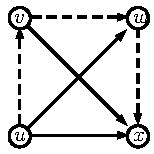
\includegraphics[scale=1.3]{TexImg/Nosubpath.pdf}
\end{figure}

\bibliographystyle{plainnat}
\bibliography{biblio}

\end{document}
